\RequirePackage[l2tabu, orthodox]{nag}
\documentclass{article}

\usepackage[letterpaper, margin=1.3cm]{geometry}
\usepackage{siunitx}
\usepackage{multicol}
\usepackage{mathtools}
\usepackage{amssymb}
\usepackage{mathrsfs}
\usepackage{graphicx}
\usepackage{float}
\usepackage[outputdir=obj]{minted}
\usepackage{pdflscape}
\usepackage{caption}
\usepackage{subcaption}
\usepackage{epstopdf}
\usepackage{filecontents}

\epstopdfsetup{outdir=./obj/}
\usemintedstyle{emacs}
\setminted{linenos,breaklines}
\begin{document}

\begin{titlepage}
	\begin{center}
		\vspace*{1cm}

		\huge{\textbf{Lab 3}}

		\vspace{0.5cm}

		\LARGE{Z-transform\\and\\Inverse Z-transform}
		\vspace{5cm}

		\Large{\textbf{Michael Kwok (1548454)}}

		\vfill
		ECE 340 Discrete Time Signals and Systems\\
		Department of Electrical and Computer Engineering\\
		University of Alberta\\
		26 October 2020
	\end{center}
\end{titlepage}
\section{Filter Response}
\subsection{Impulse response plot}
\begin{figure}[H]
	\centering
	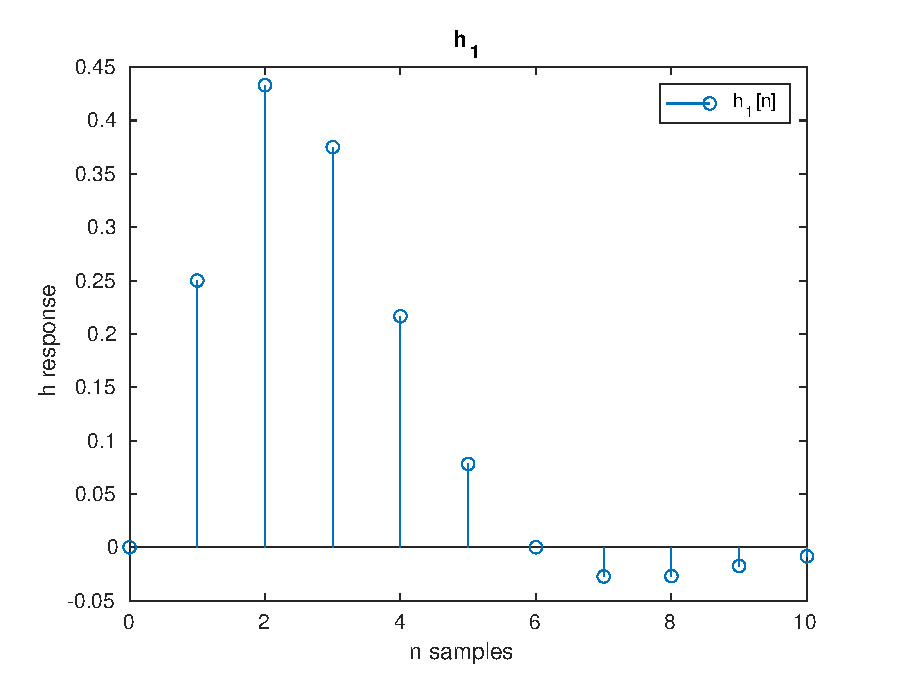
\includegraphics[width=0.4\linewidth]{h1}
	\caption{Stem plot of \(h_1[n]\)}
\end{figure}

\subsection{Z transform calculation}
Calculation and final expression for \(H(z)\):

\begin{align*}
	H(z) & = -z \frac{d}{dz}\left( \frac{\frac{z}{0.5} \sin \left(\frac{\pi}{6}\right)}{\frac{z^2}{0.25}-\frac{z}{0.25} \cos \left(\frac{\pi}{6}\right) + 1} \right) \\
	     & = -z \frac{d}{dz}\left( \frac{z\sin\left(\frac{\pi}{6}\right)}{2z^2-2z \cos\left(\frac{\pi}{6}\right) + 0.5} \right)                                      \\
	     & = \frac{2 z \sin(\frac{\pi}{6})(4z^2-1)}{{(4z^2-4\cos(\frac{\pi}{6} z + 1))}^2}                                                                           \\
	     & = \frac{4 z^3 -z}{{(4z^2 - 2 \sqrt{3} z + 1)}^2}                                                                                                          \\
	     & = \frac{4 z^{-1} - z^{-3}}{16 - 16 \sqrt{3} z^{-1} + 20 z^{-2} - 4 \sqrt{3} z^{-3} + z^{-4}}
\end{align*}


\subsection{Impulse response plot vs filter comparison}
Plot for \(h_1 \text{ vs } h_2\):

\begin{figure}[H]
	\centering
	\includegraphics[width=0.4\linewidth]{h1h2}
\end{figure}

The plots directly overlap. This makes sense as they are the same equation.

\section{Inverse Z Transform}
\subsection{Pole-Zero plots of the transfer functions}

\begin{figure}[H]
	\centering
	\begin{subfigure}[b]{0.4\linewidth}
		\centering
		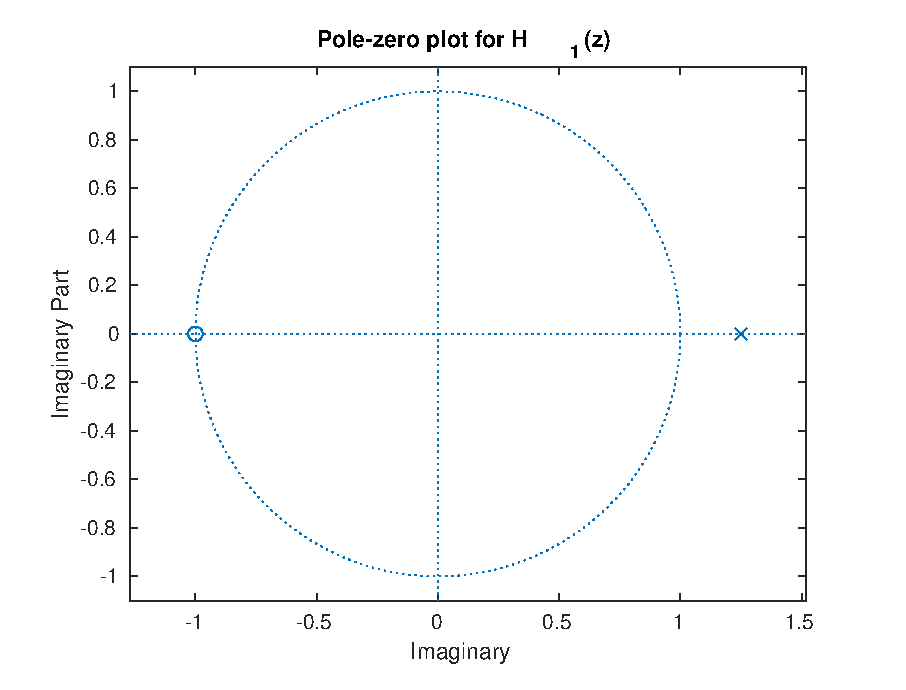
\includegraphics[width=\linewidth]{pzh1}
		\caption{\(H_1\) plot}
	\end{subfigure}
	\begin{subfigure}[b]{0.4\linewidth}
		\centering
		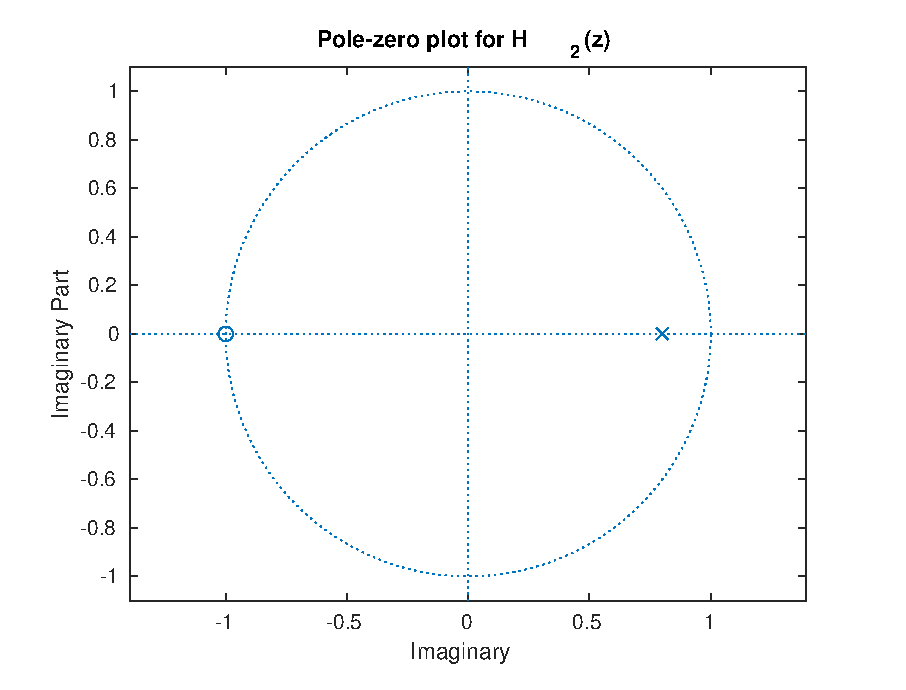
\includegraphics[width=\linewidth]{pzh2}
		\caption{\(H_2\) plot}
	\end{subfigure}
\end{figure}


The transfer functions are said to be stable, hence the pole-zero plots show that the region of convergence for \(H_1: |z| > 1.25\). Since this does not include the unit circle, \(H_1\) is unstable.

The region of convergence for \(H_2: |z| > 0.8\). This includes the unit circle, meaning \(H_2\) is stable.

\subsection{Magnitude vs Angle plot}
\begin{figure}[H]
	\centering
	\begin{subfigure}[b]{0.4\linewidth}
		\centering
		\includegraphics[width=\linewidth]{magh1}
		\caption{\(H_1\) plots}
	\end{subfigure}
	\begin{subfigure}[b]{0.4\linewidth}
		\centering
		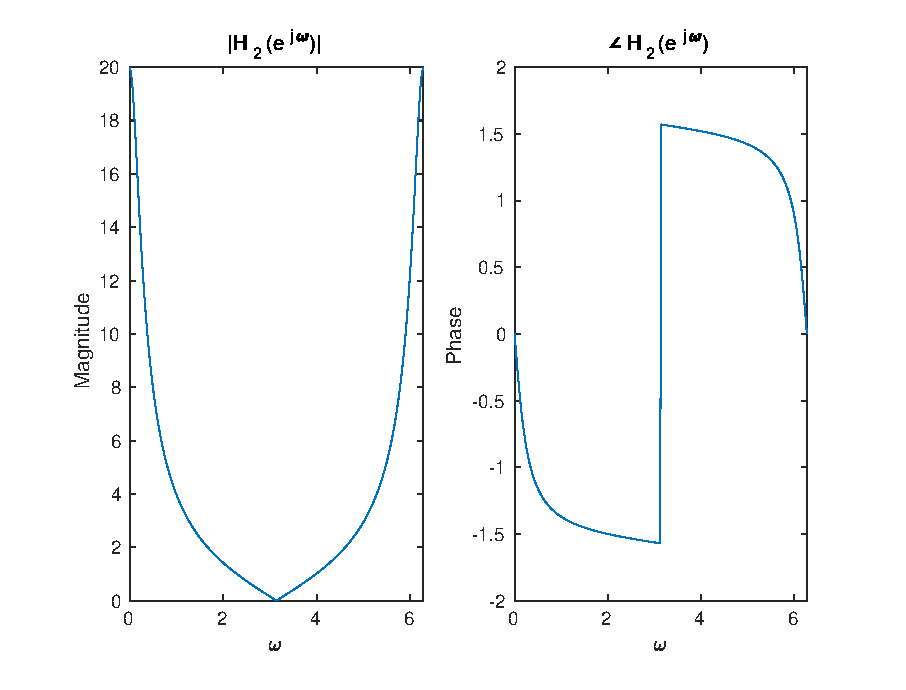
\includegraphics[width=\linewidth]{magh2}
		\caption{\(H_2\) plots}
	\end{subfigure}
\end{figure}

\subsection{Inverse Z Transform}

For \(H_1\), use ROC \(|z| > 1.25\):
\begin{align*}
	h_1 & = \frac{2}{1-1.25 z^{-1}} + \frac{2 z^{-1}}{1-1.25 z^{-1}} \\
	    & =  2\frac{z}{z-1.25} + 2 z^{-1} \frac{z}{ z- 1.25}         \\
	    & = 2(1.25^n u(n)) + 2 \left[ 1.25^{n-1} u(n-1) \right]
\end{align*}


For \(H_2\), use ROC \(|z| > 0.8\):
\begin{align*}
	h_2 & = \frac{2}{1-0.8 z^{-1}} + \frac{2 z^{-1}}{1-0.8 z^{-1}} \\
	    & =  2\frac{z}{z-0.8} + 2 z^{-1} \frac{z}{ z- 0.8}         \\
	    & = 2(0.8^n u(n)) + 2 \left[ 0.8^{n-1} u(n-1) \right]
\end{align*}

They produce the following plots:


\begin{figure}[H]
	\centering
	\begin{subfigure}[b]{0.4\linewidth}
		\centering
		\includegraphics[width=\linewidth]{imph1}
	\end{subfigure}
	\begin{subfigure}[b]{0.4\linewidth}
		\centering
		\includegraphics[width=\linewidth]{imph2}
	\end{subfigure}
\end{figure}

The resulting plots confirm the previous statement about stability. \(h_1\) grows without bounds which by definition is BIBO unstable, while \(h_2\) gets closer to 0 as n goes up which by definition is BIBO stable.
\pagebreak
\appendix
\section{Complete Code}
\inputminted{Matlab}{lab3.m}
\end{document}
